\documentclass[border=4pt]{standalone}

\usepackage{tikz} 
\usetikzlibrary{shapes,arrows,positioning,automata,backgrounds,calc,er,patterns}
\usepackage{tikz-feynman}
\tikzfeynmanset{compat=1.0.0}
 \usepackage{physics}
 
  %Use LuaLaTex to compile
\begin{document}
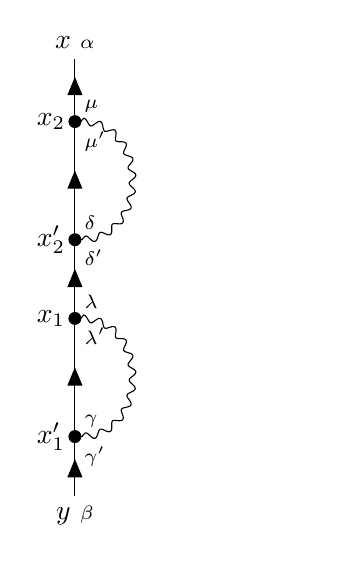
\begin{tikzpicture}
  \begin{feynman}
    %vertical
    \vertex (x) at (0,6) {\(x\) {\scriptsize \( \alpha \)}};
    \vertex [dot] (x2) at (0, 5) {};
    \vertex [dot] (x2p) at (0,3.5) {};   
    \vertex [dot] (x1) at (0, 2.5) {};     
    \vertex [dot] (x1p) at (0, 1) {};
    \vertex (y) at (0, 0) {\(y\) {\scriptsize \( \beta \)}};
    \vertex (inutile) at (3,4) {};    %just to have the four figure of the same dimension      
    \diagram*
        { 
          (y)  -- [fermion] (x1p) -- [boson, half right] (x1),   
          (x1p) -- [fermion] (x1),      
	  (x1)  -- [fermion] (x2p) -- [boson, half right] (x2),  
	  (x2p) -- [fermion] (x2),      	               
          (x2) -- [fermion] (x),
        };
  \end{feynman}
  \node[left] at (x1p) {\(x_1'\)};
  \node[left] at (x1) {\(x_1\)};  
  \node[above right] at (x1p) {{\scriptsize \( \gamma \)}};
  \node[below right] at (x1p) {{\scriptsize \( \gamma' \)}};    
  \node[above right] at (x1) {{\scriptsize \( \lambda \)}};
  \node[below right] at (x1) {{\scriptsize \( \lambda' \)}};
  
  \node[left] at (x2p) {\(x_2'\)};
  \node[left] at (x2) {\(x_2\)};  
  \node[above right] at (x2p) {{\scriptsize \( \delta \)}};
  \node[below right] at (x2p) {{\scriptsize \( \delta' \)}};    
  \node[above right] at (x2) {{\scriptsize \( \mu \)}};
  \node[below right] at (x2) {{\scriptsize \( \mu' \)}};      
\end{tikzpicture}

\end{document}
%edge label=\(x_1\)